% This work is licensed under the Creative Commons Attribution-NonCommercial 4.0 International License.
% To view a copy of this license, visit http://creativecommons.org/licenses/by-nc/4.0/
% or send a letter to Creative Commons, PO Box 1866, Mountain View, CA 94042, USA.

% !TEX TS-program = xelatex

\documentclass[../Main/chem532-notes.tex]{subfiles}
\begin{document}

\setcounter{chapter}{5}

\chapter{Molecular properties and characterization of stationary points}

\section{Density matrices and molecular properties}
In this section we will discuss the information that can be extracted from the wave function.
One of the simplest and most fundamental quantities that we can compute from the full $N$-electron wave function is the \textbf{electron density} $\rho(x_1)$, also called the \textbf{one-body density}
\begin{equation}
\rho(x_1) = N \int dx_2 \cdots dx_N \Psi(x_1,x_2,\ldots,x_N)^* \Psi(x_1,x_2,\ldots,x_N).
\end{equation}
The electron density is multiplied by $N$ so that the integral over all space is the total number of electrons
\begin{equation}
\int dx_1 \rho(x_1) = N.
\end{equation}
In addition to the electron density, we can define the one-electron density matrix $\gamma(x_1';x_1)$:\mnote{Note that the one-electron density matrix depends on two variables: $x_1$ and $x_1'$.}
\begin{equation}
\gamma(x_1';x_1) = N \int dx_2 \cdots dx_N \Psi(x_1',x_2,\ldots,x_N)^* \Psi(x_1,x_2,\ldots,x_N).
\end{equation}
The electron density can be obtainef from the one-electron density matrix by setting $x'_1$ equal to $x_1$
\begin{equation}
\rho(x_1) = \gamma(x_1;x_1),
\end{equation}
that is, the density is the diagonal component of the density matrix.

Given a one-electron operator $\hat{O}_1$, defined as:
\begin{equation}
\hat{O}_1(x) = \sum_i^N \hat{o}(x_i),
\end{equation}
the expectation value of $\hat{O}_1$ may be obtained from the one-particle density matrix.
To see this let us compute the expectation value:
\begin{equation}
\bra{\Psi}\hat{O}_1 \ket{\Psi}
= \sum_i^N  \int dx_1 \cdots dx_N \Psi(x_1,x_2,\ldots,x_N)^* \hat{o}(x_i) \Psi(x_1,x_2,\ldots,x_N).
\end{equation}
Consider one element of this sum with the operator $\hat{o}(x_i)$.
It is easy to show that it may be written in terms of the one-electron density matrix by relabeling the  coordinates $x_1 \leftrightarrow x_i$, then using the anti-symmetry of the wave function, and lastly, by introducing the auxiliary variable $x_1'$
\begin{equation}
\begin{split}
&\int dx_1 \cdots dx_N \Psi^*(x_1,\ldots,x_i,\ldots) \hat{o}(x_i) \Psi(x_1,\ldots,x_i,\ldots) \\
&= \int dx_1 \cdots dx_N \Psi^*(x_i,\ldots,x_1,\ldots) \hat{o}(x_1) \Psi(x_i,\ldots,x_1,\ldots)\\
&= \int dx_1 \cdots dx_N \Psi^*(x_1,\ldots,x_i,\ldots) \hat{o}(x_1) \Psi(x_1,\ldots,x_i,\ldots)\\
&= \int dx_1 \left[ \hat{o}(x_1) \int dx_2 \cdots dx_N \Psi^*(x_1',\ldots,x_i,\ldots)^* \Psi(x_1,\ldots,x_i,\ldots) \right]_{x_1' = x_1}\\
&= \frac{1}{N} \int dx_1 \left[ \hat{o}(x_1) \gamma(x_1';x_1) \right]_{x_1' = x_1}.
\end{split}
\end{equation}
Here we take advantage of the fact that we can relabel electron indices, and that if we simultaneously permute indices in the $\Psi^*$ and $\Psi$ functions the overall permutation factor is one. In considering the action of $\hat{o}(x_1)$ onto the product $\Psi^* \Psi$ we have to be careful to consider that $\hat{o}(x_1)$ only acts on the term on the right $\Psi$. This can be easily accounted for if we introduce an auxiliary variable $x_1'$ which, after the application of $\hat{o}(x_1)$ to $\Psi^* \Psi$, we set equal to $x_1$.
This result allows us to write:
\begin{equation}
\bra{\Psi}\hat{O}_1 \ket{\Psi}
= \int dx_1 \left[ \hat{o}(x_1) \gamma(x_1';x_1) \right]_{x_1' = x_1}.
\end{equation}

For a single Slater determinant it is possible to show that the density matrix is given by:
\begin{equation}
\gamma(x_1';x_1) = \sum_i^N \psi_i^*(x_1') \psi_i(x_1),
\end{equation}
so that the expectation value of a one-electron operator is equal to:
\begin{equation}
\begin{split}
\bra{\Psi}\hat{O}_1 \ket{\Psi}
=&
\int dx_1 \left[ \hat{o}(x_1) \sum_i^N \psi_i^*(x_1') \psi_i(x_1) \right]_{x_1' = x_1} \\
=&  \sum_i^N \int dx_1 \left[\psi_i^*(x_1') \hat{o}(x_1) \psi_i(x_1) \right]_{x_1' = x_1} \\
=&  \sum_i^N \bra{\psi_i}\hat{o}\ket{\psi_i}.
\end{split}
\end{equation}
Note that this result is consistent with the energy expression for a Slater determinant. If we substitute $\hat{o}(x_1)$ for the one-electron Hamiltonian $\hat{h}$ we recover the first contribution to the energy of a determinant.

\begin{example}[Dipole moment]
Consider the expectation value of the dipole moment operator $\hat{\boldsymbol{\mu}} = q \vec{r}$. For a molecule with $N$ electrons and $M$ nuclei
\begin{equation}
\hat{\boldsymbol{\mu}} = \sum_i^N \hat{\boldsymbol{\mu}}_i + \sum_A^M \hat{\boldsymbol{\mu}}_A = -e \sum_i^N \vec{r}_i + e \sum_A^M Z_A \vec{R}_A.
\end{equation}
The expectation value of the dipole moment operator for a single Slater determinant $\ket{\Phi} = \ket{\psi_1 \cdots \psi_N}$ is
\begin{equation}
\begin{split}
\bra{\Phi} \hat{\boldsymbol{\mu}} \ket{\Phi}
&=-e \bra{\Phi} \sum_i^N \vec{r}_i  \ket{\Phi} 
+ e \sum_A^M Z_A \vec{R}_A \braket{\Phi|\Phi}\\
&= -e \sum_i^N \bra{\psi_i}\vec{r}\ket{\psi_i} + e \sum_A^M Z_A \vec{R}_A.
\end{split}
\end{equation}

Let us expand the orbitals in the computational basis $\{\chi_\mu\}$ and integrate over the spin variable $\omega$. Then the electronic contribution reads:
\begin{equation}
\begin{split}
\sum_i^N \bra{\psi_i}\vec{r}\ket{\psi_i}
&= \sum_i^N \sum_{\mu\nu}^{K} \bra{\chi_\mu}\vec{r}\ket{\chi_\nu} C_{\mu i}^* C_{\nu i}\\
&= \sum_{\mu\nu}^{K} \bra{\chi_\mu}\vec{r}\ket{\chi_\nu} \underbrace{\sum_i^N C_{\mu i}^* C_{\nu i}}_{P_{\mu\nu}}\\
&= \sum_{\mu\nu}^{K} \bra{\chi_\mu}\vec{r}\ket{\chi_\nu} P_{\mu\nu}\\
&= \sum_\mu^K (\vec{\mathbf{r}}\,\mathbf{P}^*)_{\mu\mu} = \mathrm{Tr}(\vec{\mathbf{r}}\,\mathbf{P}^*),
\end{split}
\end{equation}
where $\mathbf{r}$ is the matrix representation of the position operator in the computational basis:
\begin{equation}
(\vec{\mathbf{r}})_{\mu\nu} = \bra{\chi_\mu}\vec{r}\ket{\chi_\nu}.
\end{equation}
Notice that $P_{\mu\nu}$ is the same density matrix that we introduced in the Hartree--Fock method.
\end{example}

Another important quantity that can be extracted from the wave function is the two-electron density ($\rho_2$), defined as
\begin{equation}
\rho_2(x_1,x_2) = \frac{N(N-1)}{2} \int dx_3 \cdots dx_N \Psi(x_1,x_2,\ldots,x_N)^* \Psi(x_1,x_2,\ldots,x_N).
\end{equation}
This quantity gives the probability of finding a pair of electrons in positions $x_1$ and $x_2$, and therefore contains information about the correlated motion of electrons.
We will see this quantity again when we will study density functional theory.
An analogous two-body density matrix can also be defined
\begin{equation}
\gamma_2(x_1,x_2; x'_1,x'_2) = \frac{N(N-1)}{2} \int dx_3 \cdots dx_N \Psi(x'_1,x'_2,\ldots,x_N)^* \Psi(x_1,x_2,\ldots,x_N),
\end{equation}
which reduces to the two-electron density when the primed coordinates are equal to the unprimed ones
\begin{equation}
\rho_2(x_1,x_2) = \gamma_2(x_1,x_2; x_1,x_2).
\end{equation}


\section{Atomic charges and bond order}

In the case of a single Slater determinant, we can perform a simple analysis of the distribution of electrons following an approach developed by Mulliken.
Recall that $i$-th MO can be expanded in terms of the AOs ($\chi_\mu$ = AO) and the coefficient matrix ($C_{\mu i}$) as:
\begin{equation}
\phi_i(\mathbf{r}) = \sum_\mu^{N} \chi_\mu(\mathbf{r}) C_{\mu i}.
\end{equation}
Since each MO is normalized we can write:\mnote{Recall that in quantum mechanics $|\Psi|^2 = \Psi^* \Psi$ is a probability density.}
\begin{equation}
\begin{split}
N =\int d\mathbf{r} \; \rho(\mathbf{r}) =  & \sum_i^{\mathrm{occ}} \braket{\psi_i | \psi_i} = 
\sum_i^{\mathrm{occ}} \sum_{\mu \nu}^N C_{\mu i}^*  \underbrace{\braket{\chi_\mu | \chi_\nu}}_{S_{\mu\nu}} C_{\nu i} \\
= & \sum_{\mu \nu}^N  S_{\mu\nu} \underbrace{\sum_i^{\mathrm{occ}}  C_{\mu i} C_{\mu i}^*}_{D_{\nu\mu}} 
= \sum_{\mu \nu}^N  S_{\mu\nu} D_{\nu\mu} = \sum_{\mu}^N  (SD)_{\mu\mu}
\end{split}
\end{equation}
\mnote{To simplify the notation we will write $\sum_{\mu} \sum_{\substack{\nu\\ \nu \neq \mu}}$ as $\sum_{\mu \neq \nu}$ and omit the superscript $N$.}


%\begin{example}[Electron density for the first and second MOs of the allyl radical]
%
%\begin{center}
%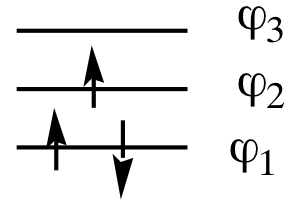
\includegraphics[width=1in]{../huckel/c2_allyl_ediagram.png}
%\end{center}
%
%For $\psi_1$
%\begin{center}
%\begin{tabular}{@{} lcr @{}} % Column formatting, @{} suppresses leading/trailing space
%\toprule
%AO & MO Coefficient ($C_{\mu i}$) & Electron density ($q^i_\mu = |C_{\mu i}|^2$)\\
%\midrule
%1 & $C_{11} = -0.5$ & $q_{1}^{1} = 0.25$ \\
%2 & $C_{21} = -0.7071$ & $q_{2}^{1} = 0.5$ \\
%3 & $C_{31} = -0.5$ & $q_{3}^{1} = 0.25$ \\
%\midrule
%Sum & & $\displaystyle \sum_{\mu = 1}^{N} q^1_\mu = 1.0$ \\
%\bottomrule
%\end{tabular}
%\end{center}
%
%For $\psi_2$
%\begin{center}
%\begin{tabular}{@{} lcr @{}} % Column formatting, @{} suppresses leading/trailing space
%\toprule
%AO & MO Coefficient ($C_{\mu i}$) & Electron density ($q^i_\mu = |C_{\mu i}|^2$)\\
%\midrule
%1 & $C_{12} = 0.7071$ & $q_{1}^{2} = 0.5$ \\
%2 & $C_{22} = 0$ & $q_{2}^{2} = 0$ \\
%3 & $C_{32} = -0.7071$ & $q_{3}^{2} = 0.5$ \\
%\midrule
%Sum & & $\displaystyle \sum_{\mu = 1}^{N} q^2_\mu = 1.0$ \\
%\bottomrule
%\end{tabular}
%\end{center}
%\end{example}


Using these quantities we define:
\begin{itemize}
\item \textbf{Total density on atom} $\mu$ ($q_\mu$):
\begin{equation}
q_\mu = \sum_{i}^{\rm MO} n_i |C_{\mu i}|^2 = \sum_{i}^{\rm MO} n_i q_\mu^i \quad n_i \text{ = occupation (2, 1, or 0)} 
\end{equation}

\item \textbf{Total charge on atom} $\mu$ ($N_\mu$):
\begin{equation}
N_\mu = (\text{number of $\pi$ electrons donated by atom $\mu$}) - q_\mu
\end{equation}

\item \textbf{Total bond order between atoms  $\mu$ and  $\nu$} ($p_{\mu \nu}$):
\begin{equation}
p_{\mu \nu}= \sum_{i}^{\rm MO} n_i C_{\mu i}^* C_{\nu i} = \sum_{i}^{\rm MO} n_i p_{\mu\nu}^i
\end{equation}
\end{itemize}



\section{Energy gradients}
Another useful property that we would like to extract from quantum chemistry computations is the gradient of the energy with respect to the position of the nuclei ($R_\alpha$):
\begin{equation}
g_\alpha(\mathbf{R}) = \frac{\partial V(\mathbf{R})}{\partial R_\alpha} \quad \alpha = 1,\ldots,3M.
\end{equation}
Energy gradients can be obtained either by using numeral methods, for example, by taking finite differences of the energy, or by analytical methods that directly compute the gradients of the energy.

In the finite difference method, the gradient and second derivatives are computed by repeatedly evaluating the energy at different geometries around a reference geometry $\mathbf{R}_0$.
Suppose we are interested in computing the gradient of a function $f(x)$ at a point $x_0$. In the finite difference method we expand $f(x)$ as a Taylor series at a point $x_0 + h$, where $h$ is a small displacement
\begin{equation}
f(x_0 + h) = f(x_0) + f'(x_0) h + \frac{1}{2} f''(x_0) h^2 + O(h^3),
\end{equation},
from which we can obtain $f'(x_0)$
\begin{equation}
f'(x_0) = \frac{f(x_0 + h) -f(x_0)}{h} - \frac{1}{2} f''(x_0) h + O(h^2).
\end{equation}
For a sufficiently small value of $h$ we can write
\begin{equation}
f'(x_0) = \frac{f(x_0 + h) -f(x_0)}{h} + O(h),
\end{equation}
which shows that the error in the gradient is proportional to $h$.
A more accurate finite difference scheme may be obtained by considering the Taylor series centered around $x_0 - h$
\begin{equation}
f(x_0 - h) = f(x_0) - f'(x_0) h + \frac{1}{2} f''(x_0) h^2 + O(h^3),
\end{equation}
and subtracting this from the expression for $f(x_0 + h)$
\begin{equation}
f(x_0 + h) - f(x_0 - h) = 2 f'(x_0) h + O(h^3).
\end{equation}
From this expression we get an estimate of the gradient with an error that in now proportional to order $h^2$
\begin{equation}
f'(x_0) = \frac{f(x_0 + h) - f(x_0 - h)}{2h} + O(h^2).
\end{equation}
Analogous formulas can be obtained to determine the energy with higher accuracy. For example, the following equation provides the gradient approximate to order $h^4$
\begin{equation}
f'(x_0) = \frac{-f(x_0 + 2h) + 8 f(x_0 + h)- 8f(x_0 - h) + f(x_0 - 2h)}{12h} + O(h^4).
\end{equation}
These equations may be generalized to second derivative and to the case where there is more than one variable.

The theory behind analytical gradients is well established but highly technical, so it will not be covered in these notes. In general, the cost to compute analytical gradients is similar to that of an energy evaluation. Compare this to the cost of computing the gradient via finite difference, where for each direction ($3M-5$ or $3M-6$) we have to compute 2, 4, or more energies to obtain the gradient.
The numerical method is clearly more expensive, but sometimes it is the only option available because the analytical gradients may have not been developed and implemented.

\section{Stationary points and geometry optimization}
Gradients are important because they allow us to find stationary points of the potential energy surface $E(\mathbf{R})$.
Stationary points are defined as those geometries ($\tilde{\mathbf{R}}$) for which all gradients are zero:
\begin{equation}
g_\alpha(\tilde{\mathbf{R}}) = 0 \quad \alpha = 1,\ldots,3M.
\end{equation}
A stationary point can be found by an optimization algorithm like the Newton--Raphson method. 

\begin{example}[Newton--Raphson method in one dimension]
In one dimension the gradient is a scalar $g$.
If we expand the potential around an arbitrary point $x_0$ in a Taylor expansion
\begin{equation}
\begin{split}
V(x) &= V(x_0) + \left.\frac{dV(x)}{dx}\right|_{x = x_0} (x - x_0)
+ \frac{1}{2!} \left.\frac{d^2V(x)}{dx^2}\right|_{x = x_0} (x - x_0)^2 + \ldots \\
&= V(x_0) + g_0 (x - x_0)
+ \frac{1}{2!} h_0 (x - x_0)^2 + \ldots,
\end{split}
\end{equation}
where $g_0 = \left.\frac{dV(x)}{dx}\right|_{x = x_0}$ and $h_0 = \left.\frac{d^2V(x)}{dx^2}\right|_{x = x_0}$ are the gradient and hessian, respectively.

To find a stationary point we need to impose $\frac{dV(x)}{dx} = 0$. Differentiating the Taylor expansion once we obtain
\begin{equation}
\frac{dV(x)}{dx} = g_0 + h_0 (x - x_0) + \ldots.
\end{equation}
Neglecting the terms quadratic in $(x - x_0)$ and imposing $\frac{dV(x)}{dx} = 0$ we get:
\begin{equation}
g_0 + h_0 (x - x_0) = 0,
\end{equation}
or:
\begin{equation}
x = x_0 - \frac{g_0}{h_0}.
\end{equation}
Thus we can find an approximation to the stationary point using the gradient and the Hessian of the energy.
If we apply this equation we are unlikely to land right away onto the stationary point, and an iterative procedure is usually required.
\end{example}

For a general molecule, we can derive the Newton--Raphson method by expanding the energy $V(\mathbf{R})$ as a Taylor series
\begin{equation}
\begin{split}
V(\mathbf{R}) =& V(\mathbf{R}_0)
+ \sum_\alpha^{3M} \left.\frac{\partial  V}{\partial R_\alpha}\right|_{\mathbf{R} = \mathbf{R}_0} \Delta R_\alpha \\
&+ \frac{1}{2!} \sum_{\alpha\beta}^{3M}\left.\frac{\partial^2 V}{\partial R_\alpha \partial R_\beta}\right|_{\mathbf{R} = \mathbf{R}_0} \Delta R_\alpha \Delta R_\beta + \ldots \\
=& V(\mathbf{R}_0)
+ \mathbf{g}^{T} \Delta \mathbf{R} + \frac{1}{2} \Delta\mathbf{\mathbf{R}}^{T} \mathbf{F} \Delta \mathbf{R} + \ldots,
\end{split}
\end{equation}
where we introduced the displacement vector $(\Delta\mathbf{\mathbf{R}})\alpha = \Delta R_\alpha = R_\alpha - R_{0,\alpha}$, the gradient vector
\begin{equation}
g_\alpha = \frac{\partial  V}{\partial R_\alpha},
\end{equation}
and the Hessian matrix (force constant):
\begin{equation}
F_{\alpha\beta} = \frac{\partial^2 V}{\partial R_\alpha R_\beta}.
\end{equation}
The gradient of $V(\mathbf{R})$ is then
\begin{equation}
\nabla V(\mathbf{R}) = \mathbf{g} + \mathbf{F} \Delta \mathbf{R} + \ldots,
\end{equation}
and imposing $\nabla V(\mathbf{R}) = 0$ we get (after neglecting higher-order terms):
\begin{equation}
\Delta \mathbf{R} = -\mathbf{F}^{-1} \mathbf{g},
\end{equation}
or
\begin{equation}
\mathbf{R} = \mathbf{R}_0 - \mathbf{F}^{-1} \mathbf{g}.
\end{equation}
This procedure for optimizing the geometry is called the Newton--Raphson method.
It requires both the energy gradient ($\mathbf{g}$) and the Hessian ($\mathbf{F}$).
In a typical quantum chemistry code the Hessian might not be computed exactly. Instead, one may start from a guess and update the Hessian with information from the gradient as one explores the potential energy surface during an optimization.

\section{Normal Coordinate Analysis and Harmonic Frequencies}
Once we identify a stationary point, it is possible to characterize its nature (minimum, saddle point, maximum) by performing a normal mode analysis.
In a normal mode analysis we will solve the nuclear Schr\"{o}dinger equation at a minimum geometry by expanding the potential up to quadratic terms.
Recall that the nuclear Schr\"{o}dinger equation in the Born--Oppenheimer approximation is:
\begin{equation}
\hat{H}_{{\rm nuc}} \chi_{v}(\mathbf{R}) =  E_{v} \chi_{v}(\mathbf{R}),
\end{equation}
where $\hat{H}_{{\rm nuc}}$ is the nuclear Hamiltonian for a given electronic state (we omit the index $k$ to simply the notation)
\begin{equation}
\hat{H}_{{\rm nuc}} = \hat{T}_{N} + V(\mathbf{R}).
\end{equation}
For small vibrations around a minimum (or any other type of stationary point), the potential can be expanded up to quadratic terms as
\begin{equation}
V(\mathbf{R}) \approx V(\mathbf{R}_0)
+ \frac{1}{2} \Delta\mathbf{\mathbf{R}}^{T} \mathbf{F} \Delta \mathbf{R}
= V(\mathbf{R}_0) + 
\frac{1}{2!} \sum_{\alpha\beta}^{3M}  \Delta R_\alpha F_{\alpha\beta} \Delta R_\beta,
\end{equation}
while the kinetic energy operator (in atomic units) is:
\begin{equation}
\hat{T}_N = -\frac{1}{2} \sum_\alpha^{3M} \frac{1}{M_\alpha} \frac{\partial^2}{\partial R_\alpha^2}.
\end{equation}

Unfortunately, the potential couples different atomic Cartesian coordinates together, which prevents a direct solution of the Schr\"{o}dinger equation.
To solve this problem we first rewrite the kinetic energy operators in terms of Cartesian displacements. Using the chain rule we can show that taking the derivative with respect to a coordinate $R_\alpha$ is equivalent to taking the derivative with respect to its corresponding displacement $ \Delta R_\alpha$
\begin{equation}
\frac{\partial}{\partial R_\alpha}
= \sum_\beta \frac{\partial \Delta R_\beta}{\partial R_\alpha} \frac{\partial }{\partial \Delta R_\beta}
= \sum_\beta \delta_{\alpha\beta} \frac{\partial }{\partial \Delta R_\beta}
= \frac{\partial }{\partial \Delta R_\alpha}.
\end{equation}
Using Cartesian displacements, the Hamiltonian operator may be written as
\begin{equation}
\hat{H}_\mathrm{nuc} = -\frac{1}{2} \sum_\alpha^{3M} \frac{1}{M_\alpha} \frac{\partial^2}{\partial \Delta R_\alpha^2}
+ \frac{1}{2} \sum_{\alpha\beta}^{3M} \Delta R_\alpha F_{\alpha\beta} \Delta R_\beta.
\end{equation}
Next, we want to hide the mass dependence. To this end, introduce mass-weighted  coordinates ($q_\alpha$), defined as
\begin{equation}
q_\alpha = \sqrt{M_\alpha} \Delta R_\alpha.
\end{equation}
With this transformation the derivative with respect to $\Delta R_\alpha$ may be written as
\begin{equation}
\frac{\partial }{\partial \Delta R_\alpha}
= \sum_\beta \frac{\partial q_\beta}{\partial \Delta R_\alpha} \frac{\partial}{\partial q_\beta}
= \sum_\beta \sqrt{M_\beta} \delta_{\alpha\beta} \frac{\partial}{\partial q_\beta} = \sqrt{M_\alpha} \frac{\partial}{\partial q_\alpha}.
\end{equation}
Plugging in this result into the Hamiltonian we get
\begin{equation}
\hat{H}_\mathrm{nuc} = -\frac{1}{2} \sum_\alpha^{3M} \frac{\partial^2}{\partial q_\alpha^2}
+ \frac{1}{2} \sum_{\alpha\beta}^{3M} q_\alpha \tilde{F}_{\alpha\beta} q_\beta,
\end{equation}
where $\tilde{F}_{\alpha\beta}$ is the mass-weighted Hessian:
\begin{equation}
\tilde{F}_{\alpha\beta} = \frac{F_{\alpha\beta}}{\sqrt{M_\alpha M_\beta}}.
\end{equation}
If we introduce the diagonal mass matrix $\mathbf{W}$:
\begin{equation}
W_{\alpha\beta} = M_\alpha \delta_{\alpha\beta},
\end{equation}
we can write the mass-weighted Hessian as:
\begin{equation}
\tilde{\mathbf{F}} = \mathbf{W}^{-1/2} \mathbf{F} \mathbf{W}^{-1/2}
\end{equation}


The last step consists in diagonalizing the mass-weighted Hessian. Consider the orthogonal matrix $\mathbf{L}$ that diagonalizes $\tilde{\mathbf{F}}$:
\begin{equation}
\tilde{\mathbf{F}}\mathbf{L} = \mathbf{L}\boldsymbol{\lambda}.
\end{equation}
If we express the mass-weighted Hessian as $\tilde{\mathbf{F}} = \mathbf{L}\boldsymbol{\lambda}\mathbf{L}^{T}$, we can rewrite the potential energy term as:
\begin{equation}
\frac{1}{2} \sum_{\alpha\beta\gamma}^{3M} q_\alpha  L_{\alpha\gamma} \lambda_\gamma L_{\beta\gamma} q_\beta
= \frac{1}{2} \sum_{\gamma}^{3M} (\sum_{\alpha} q_\alpha  L_{\alpha\gamma})\lambda_\gamma (\sum_{\beta} q_\beta L_{\beta\gamma}),
\end{equation}
which suggests introducing a new set of variables, the normal modes ($Q_\gamma$):
\begin{equation}
Q_\gamma = \sum_{\alpha} q_\alpha  L_{\alpha\gamma}.
\end{equation}
Since $\mathbf{L}$ is an orthogonal transformation, the structure of the kinetic energy operator does not change when transforming the coordinate systems. Hence, we can finally write the Hamiltonian as
\begin{equation}
\hat{H}_\mathrm{nuc} = -\frac{1}{2} \sum_\alpha^{3M} \frac{\partial^2}{\partial Q_\alpha^2} + \frac{1}{2} \sum_\alpha^{3M} \lambda_\alpha Q_\alpha^2
= \sum_\alpha^{3M} \left[
-\frac{1}{2} \frac{\partial^2}{\partial Q_\alpha^2} + \frac{1}{2} \lambda_\alpha Q_\alpha^2
\right].
\end{equation}

Note that in the normal coordinate system the potential is a quadratic function:
\begin{equation}
V(\mathbf{Q}) = \sum_\alpha^{3M} \lambda_\alpha Q_\alpha^2.
\end{equation}
Therefore, if all $\lambda_\alpha$ are positive ($\lambda_\alpha > 0$), then the stationary point is a minimum.
If one or more $\lambda_\alpha < 0$ we have a saddle point.
If all $\lambda_\alpha < 0$ then we are at a maximum.
Thus, a harmonic vibrational analysis can be used after geometry optimization to characterize the nature of a stationary point.
Note that for saddle points and maxima the concept of vibrational frequency breaks down because we have to take the square root of a negative number.
In this case we talk about \textbf{imaginary frequencies}.
Minima are said to have no imaginary frequencies.

In the normal mode coordinates, the Hamiltonian is a sum of terms of the form
\begin{equation}
\hat{H}_\alpha = -\frac{1}{2} \frac{\partial^2}{\partial Q_\alpha^2} + \frac{1}{2} \lambda_\alpha Q_\alpha^2,
\end{equation}
which is the Hamiltonian for a harmonic oscillator with unity mass and force constant $k = \lambda_\alpha$.
The eigenvalues for this Hamiltonian are given by
\begin{equation}
E_{\alpha}^{(v_\alpha)} = \sqrt{\lambda_\alpha}\left(\frac{1}{2} + v_\alpha\right),
\end{equation}
where $v_\alpha = 0,1,\ldots$ is the vibrational quantum number for the normal mode $Q_\alpha$.
The total nuclear energy is given by:
\begin{equation}
E^{\mathbf{v}} = \sum_\alpha E_{\alpha}^{(v_\alpha)}
= \frac{1}{2} \sum_\alpha \sqrt{\lambda_\alpha}
+ \sum_\alpha \sqrt{\lambda_\alpha} v_\alpha.
\end{equation}
The first term in this expansion is the zero-point vibrational energy (ZPVE) in the harmonic approximation.
This is the energy of the nuclei in the ground vibrational state.



The normal modes may be related to the Cartesian displacements by combining all the coordinate transformations.
Starting from the normal modes one finds that: 
\begin{equation}
\mathbf{Q}^{T} = \mathbf{q}^{T} \mathbf{L} =  \Delta\mathbf{R}^{T} \mathbf{W}^{1/2}\mathbf{L}
\end{equation}
and taking the transpose:
\begin{equation}
\mathbf{Q} =  \mathbf{L}^{T} \mathbf{W}^{1/2} \Delta\mathbf{R}.
\end{equation}
Now after solving for $\Delta\mathbf{R}$ we get:
\begin{equation}
\Delta\mathbf{R} = \mathbf{W}^{-1/2}\mathbf{L} \mathbf{Q}.
\end{equation}




\end{document}

 




